\documentclass[12pt, oneside]{book}
\usepackage[a4paper,top=2.5cm,bottom=2.5cm,left=3.5cm,right=2cm]{geometry}
\usepackage[utf8]{inputenc}
\usepackage[T1]{fontenc}
\usepackage{graphicx}
\usepackage{url}
\usepackage[hidelinks,breaklinks]{hyperref}
\usepackage[english, slovak]{babel} % vypnite pre prace v anglictine
\usepackage{amsmath}
\usepackage{varwidth}

\usepackage{amsthm}

\let\eps=\varepsilon % definujeme si pekne epsilon
\newtheorem*{definition}{Definition}
\setcounter{secnumdepth}{2}

\linespread{1.25} % hodnota 1.25 by mala zodpovedat 1.5 riadkovaniu

% -------------------
% --- Definicia zakladnych pojmov
% --- Vyplnte podla vasho zadania
% -------------------
\def\mfrok{2017}
\def\mfnazov{Approximate Abundance Histograms and Their Use for Genome Size Estimation}
\def\mftyp{Bachelor Thesis}
\def\mfautor{Mário Lipovský}
\def\mfskolitel{Mgr. Bronislava Brejová, PhD.}

%ak mate konzultanta, odkomentujte aj jeho meno na titulnom liste
\def\mfkonzultant{tit. Meno Priezvisko, tit. }  

\def\mfmiesto{Bratislava, \mfrok}

%aj cislo odboru je povinne a je podla studijneho odboru autora prace
\def\mfodbor{2508 Informatics} 
\def\program{Informatics}
\def\mfpracovisko{Department of Computer Science}

\begin{document}
\selectlanguage{english}

\frontmatter


% -------------------
% --- Obalka ------
% -------------------
\thispagestyle{empty}

\begin{center}
\sc\large
Comenius University, Bratislava\\
Faculty of Mathematics, Physics and Informatics

\vfill

{\LARGE\mfnazov}\\
\mftyp
\end{center}

\vfill

{\sc\large 
\noindent \mfrok\\
\mfautor
}

\eject % EOP i
% --- koniec obalky ----

% -------------------
% --- Titulný list
% -------------------

\thispagestyle{empty}
\noindent

\begin{center}
\sc  
\large
Comenius University, Bratislava\\
Faculty of Mathematics, Physics and Informatics

\vfill

{\LARGE\mfnazov}\\
\mftyp
\end{center}

\vfill

\noindent
\begin{tabular}{ll}
Study programme: & \program \\
Study field: & \mfodbor \\
Department: & \mfpracovisko \\
Supervisor: & \mfskolitel \\
% Consultant: & \mfkonzultant \\
\end{tabular}

\vfill


\noindent \mfmiesto\\
\mfautor

\eject % EOP i


% --- Koniec titulnej strany


% -------------------
% --- Zadanie z AIS
% -------------------
% v tlačenej verzii s podpismi zainteresovaných osôb.
% v elektronickej verzii sa zverejňuje zadanie bez podpisov

\newpage 
\thispagestyle{empty}
\hspace{-3.5cm}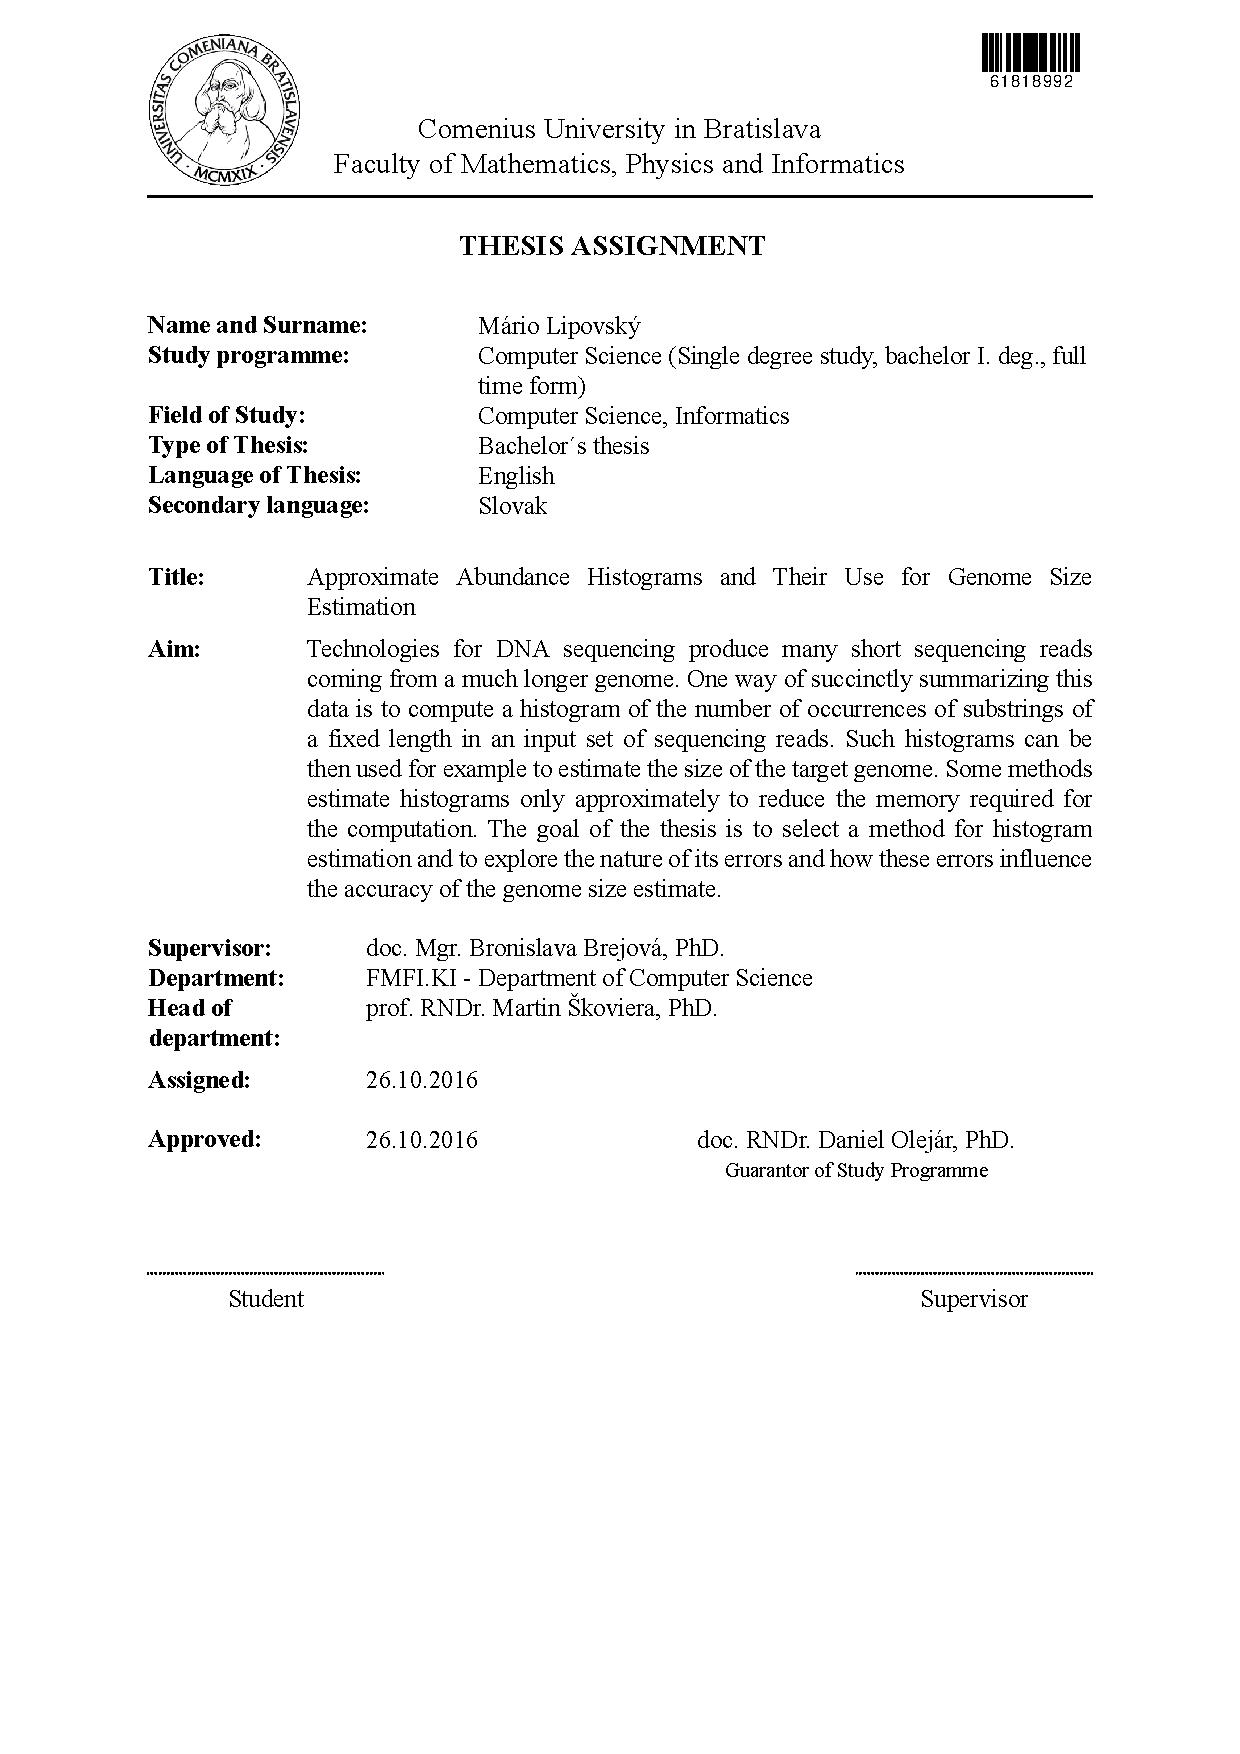
\includegraphics[width=1.3\textwidth]{images/zadanie-aj}

\newpage 
\thispagestyle{empty}
\hspace{-3.5cm}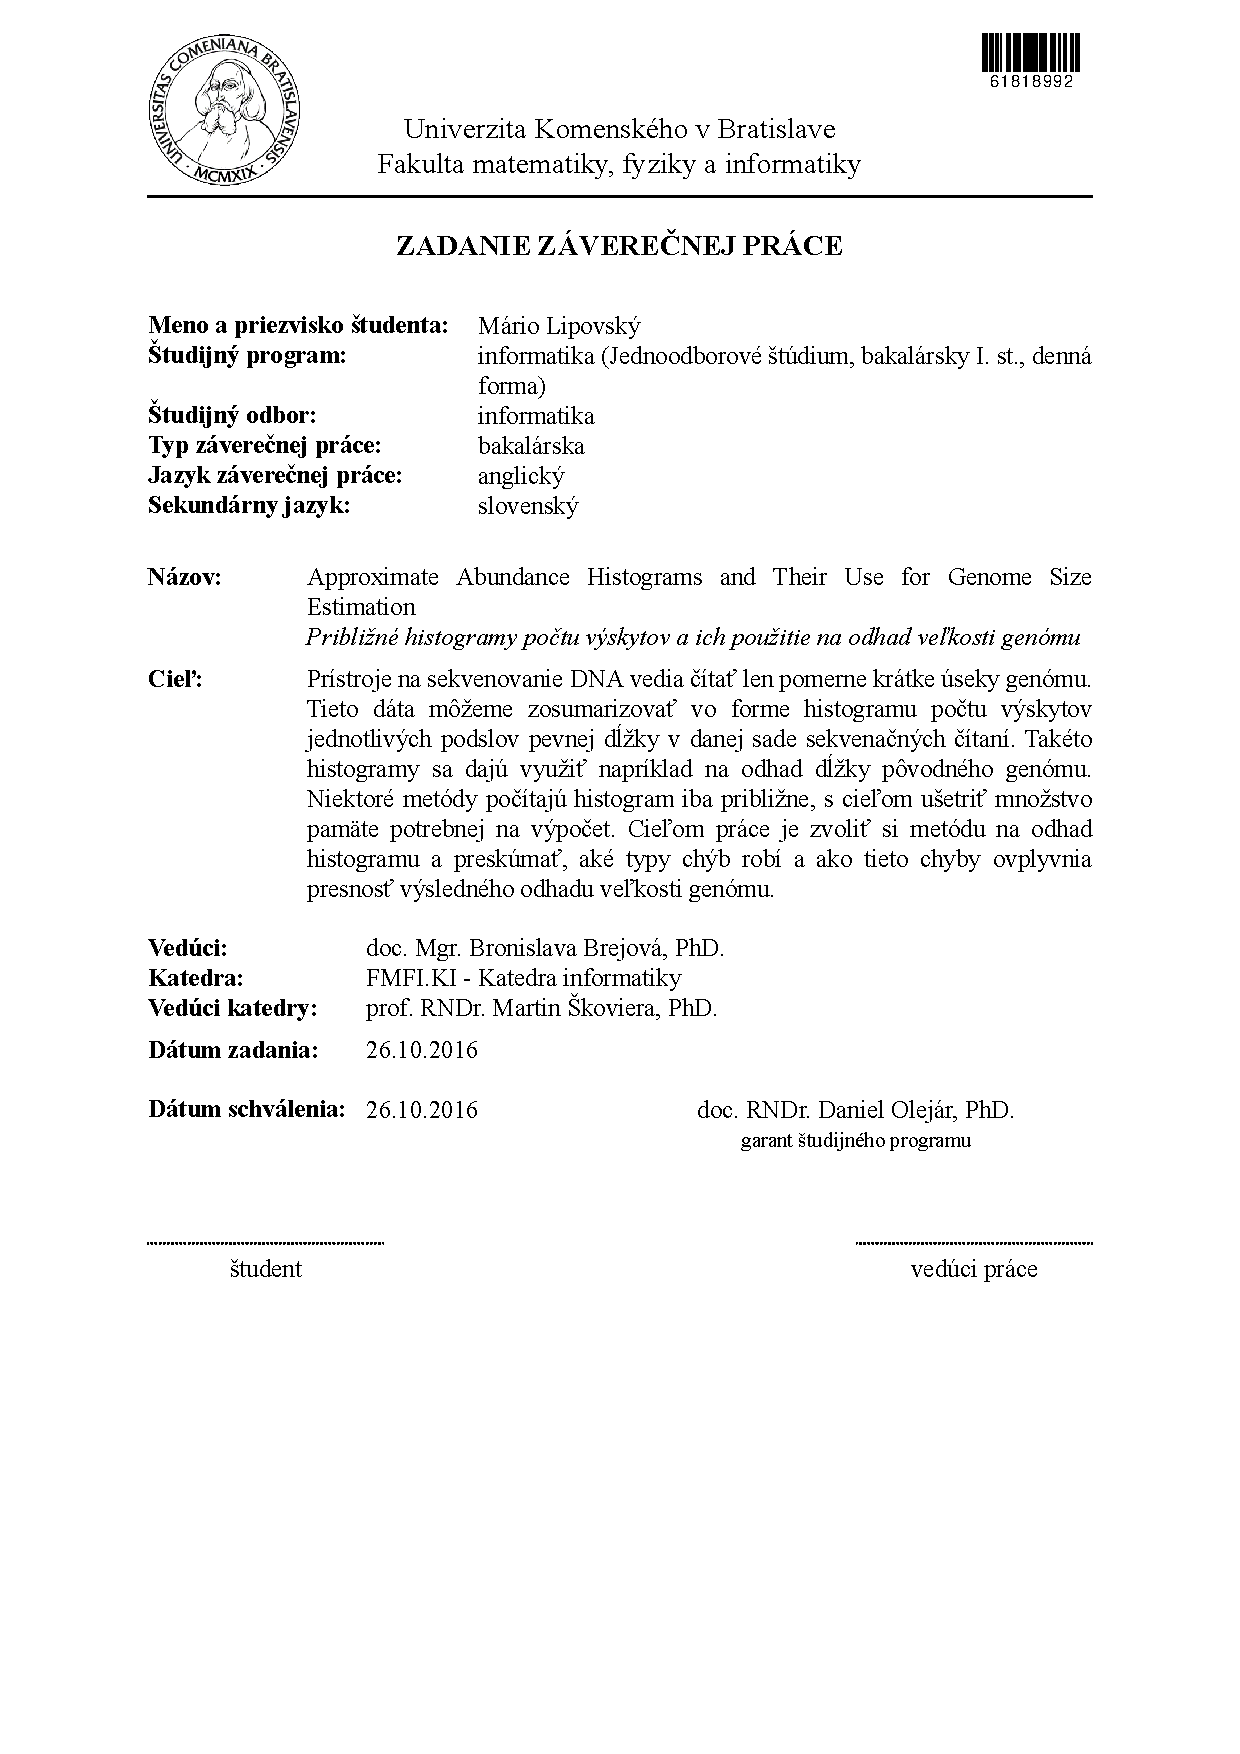
\includegraphics[width=1.3\textwidth]{images/zadanie-sj}

% --- Koniec zadania

\frontmatter

% -------------------
%   Poďakovanie - nepovinné
% -------------------
\setcounter{page}{3}
\newpage 
\chapter*{Acknowledgement}

% I would like to thank my supervisor doc. Mgr. Bronislava Brejová, PhD.
% for 

% --- Koniec poďakovania

% -------------------
%   Abstrakt - Slovensky
% -------------------
\newpage 
\chapter*{Abstrakt}
Sekvenovaním DNA zvyčajne vzniká množstvo krátkych reťazcov. 
Sekvenovacie dáta môžeme zosumarizovať vo forme histogramu počtov výskytov jednotlivých
podslov pevnej dĺžky. Takéto histogramy sa dajú použiť napríklad na odhadovanie dĺžky 
genómu. V našej práci skúmame algoritmus Kmerlight, ktorý počíta spomínaný histogram približne.
Zistili sme, že Kmerlight počíta vychýlené odhady histogramov, no podarilo sa nám navrhnúť 
novú verziu algoritmu Kmerlight, ktorej odhady sú už nevychýlené. V práci ďalej teoreticky 
modelujeme pravdepodobnostné rozdelenie chýb odhadov histogramu a pomocou experimentov 
sme overili správnosť nášho modelu. Na záver sme použili program CovEst 
na výpočet odhadov dĺžok genómov z približných histogramov a preskúmali sme, ako
chyby v histogramoch ovplyvňujú presnosť týchto odhadov. Napriek tomu, že CovEst bol
navrhnutý na spracúvanie presných histogramov, naše výsledky ukazujú, že CovEst môže byť použitý
aj na približných histogramoch, ktorých výpočet si vyžaduje menšie množstvo pamäte.


\paragraph*{Kľúčové slová:} histogram počtov $k$-tic, Kmerlight, odhad dĺžky genómu, CovEst
% --- Koniec Abstrakt - Slovensky


% -------------------
% --- Abstrakt - Anglicky 
% -------------------
\newpage 
\chapter*{Abstract}

DNA sequencing data is typically a large collection of short strings called reads.
We can summarize such data by computing a histogram of the number of occurrences of substrings of 
a fixed length. Such histograms can be used for example to estimate the size of a genome. 
In this thesis we study an existing tool, Kmerlight, which
computes approximate histograms. We discover an approximation bias, and we propose
a new, unbiased version of Kmerlight. We also model the distribution of approximation
errors, and we support our theoretical model by experimental data. Furthermore, we use another
tool, CovEst, to compute genome size estimates with use of approximate histograms, and 
we evaluate the precision of such estimates compared to results obtained from exact histograms.
Our results show that although CovEst was designed to work with exact histograms,
it can be used with their approximate versions, which can be produced in a much smaller amount of
memory.


\paragraph*{Keywords:} $k$-mer abundance histogram, Kmerlight, genome size estimation, CovEst  

% --- Koniec Abstrakt - Anglicky

% -------------------
% --- Predhovor - v informatike sa zvacsa nepouziva
% -------------------
%\newpage 
%\thispagestyle{empty}
%
%\huge{Predhovor}
%\normalsize
%\newline
%Predhovor je všeobecná informácia o práci, obsahuje hlavnú charakteristiku práce 
%a okolnosti jej vzniku. Autor zdôvodní výber témy, stručne informuje o cieľoch 
%a význame práce, spomenie domáci a zahraničný kontext, komu je práca určená, 
%použité metódy, stav poznania; autor stručne charakterizuje svoj prístup a svoje 
%hľadisko. 
%
% --- Koniec Predhovor


% -------------------
% --- Obsah
% -------------------

\newpage 

\tableofcontents

% ---  Koniec Obsahu

% -------------------
% --- Zoznamy tabuliek, obrázkov - nepovinne
% -------------------

\newpage 

\listoffigures
\listoftables

% ---  Koniec Zoznamov

\mainmatter


\input introduction.tex 

% Chapter 1
\input chapter1/biological-motivation.tex

\input chapter1/histogram-computing-methods.tex

\input chapter1/genome-size-estimation.tex

\input chapter1/problem-statement.tex

% Chapter 2
\input chapter2/kmerlight.tex

\input chapter2/errors-observation.tex

\input chapter2/source-of-bias.tex

\input chapter2/unbiased-estimation.tex

\input chapter2/variance.tex

\input chapter2/choice-of-parameters.tex

% Chapter 3
\input chapter3/covest.tex

\input chapter3/covest-and-kmerlight.tex

\input chapter3/alternative-likelihood.tex

\input conclusion.tex

% -------------------
% --- Bibliografia
% -------------------


\newpage	

\backmatter

\thispagestyle{empty}
\nocite{*}
\clearpage

\bibliographystyle{plain}
\bibliography{bibliography} 

%---koniec Referencii

% -------------------
%--- Prilohy---
% -------------------

% Nepovinná časť prílohy obsahuje materiály, ktoré neboli zaradené priamo  do textu.
% Každá príloha sa začína na novej strane.
% Zoznam príloh je súčasťou obsahu.
%
\input AppendixA.tex

%\addcontentsline{toc}{chapter}{Appendix B}
%\input AppendixB.tex

\end{document}






